\pdfminorversion=4
\documentclass[aspectratio=169]{beamer}

\mode<presentation>
{
  \usetheme{default}
  \usecolortheme{default}
  \usefonttheme{default}
  \setbeamertemplate{navigation symbols}{}
  \setbeamertemplate{caption}[numbered]
  \setbeamertemplate{footline}[frame number]  % or "page number"
  \setbeamercolor{frametitle}{fg=white}
  \setbeamercolor{footline}{fg=black}
} 

\usepackage[english]{babel}
\usepackage[utf8x]{inputenc}
\usepackage{tikz}
\usepackage{courier}
\usepackage{array}
\usepackage{bold-extra}
\usepackage{minted}
\usepackage[thicklines]{cancel}
\usepackage{fancyvrb}
\usepackage{amsmath}

\xdefinecolor{dianablue}{rgb}{0.18,0.24,0.31}
\xdefinecolor{darkblue}{rgb}{0.1,0.1,0.7}
\xdefinecolor{darkgreen}{rgb}{0,0.5,0}
\xdefinecolor{darkgrey}{rgb}{0.35,0.35,0.35}
\xdefinecolor{darkorange}{rgb}{0.8,0.5,0}
\xdefinecolor{darkred}{rgb}{0.7,0,0}
\definecolor{darkgreen}{rgb}{0,0.6,0}
\definecolor{mauve}{rgb}{0.58,0,0.82}

\title[2019-05-22-colloquium-languages]{Programming languages and particle physics}
\author{Jim Pivarski}
\institute{Princeton University -- IRIS-HEP}
\date{May 8, 2019}

%% Title: Programming languages and particle physics

%% Abstract:

%% Programming languages aren't for computers; they're for people. If a language doesn't make it easier to express your physics problem, it's not a suitable language. Some fields have specialized "Domain Specific Languages" (DSLs) that trade freedom of expression for focus on the problem at hand, and can even improve performance by limiting this scope. A prime example is SQL, widely used by data analysts outside of physics, which trades generic computation for a SELECT-WHERE-GROUPBY pattern. Interestingly, this was the design pattern of the first electromechanical computers (Hollerith machine, 1890) and it's still a major focus of big data today (Dean & Ghemawat: MapReduce, 2004). Particle physics problems don't fit SQL well; in fact, physicists became involved in computing in tandem with the invention of generic, digital computers (Von Neumann's stored-program machine, 1945). I will present some history, some general features of programming languages, what "declarative" really means, and will show some perhaps surprising examples of DSLs you're already using.

\usetikzlibrary{shapes.callouts}

\begin{document}

\logo{\pgfputat{\pgfxy(0.11, 7.4)}{\pgfbox[right,base]{\tikz{\filldraw[fill=dianablue, draw=none] (0 cm, 0 cm) rectangle (50 cm, 1 cm);}\mbox{\hspace{-8 cm}
\includegraphics[height=1 cm]{princeton-logo-long.png}\hspace{0.1 cm}\raisebox{0.1 cm}{
\includegraphics[height=0.8 cm]{iris-hep-logo-long.png}}\hspace{0.1 cm}}}}}

\begin{frame}
  \titlepage
\end{frame}

\logo{\pgfputat{\pgfxy(0.11, 7.4)}{\pgfbox[right,base]{\tikz{\filldraw[fill=dianablue, draw=none] (0 cm, 0 cm) rectangle (50 cm, 1 cm);}\mbox{\hspace{-8 cm}
\includegraphics[height=1 cm]{princeton-logo.png}\hspace{0.1 cm}\raisebox{0.1 cm}{
\includegraphics[height=0.8 cm]{iris-hep-logo.png}}\hspace{0.1 cm}}}}}

% Uncomment these lines for an automatically generated outline.
%\begin{frame}{Outline}
%  \tableofcontents
%\end{frame}

% START START START START START START START START START START START START START

\begin{frame}{}
\vspace{-0.1 cm}
\begin{columns}
\column{1.15\linewidth}

\includegraphics[width=\linewidth]{same-river-twice.jpg}
\end{columns}
\end{frame}

\begin{frame}{}
\huge
\vspace{0.5 cm}
\begin{center}
Because, you know, it's different water.
\end{center}
\end{frame}

\begin{frame}{Why do we say it's the same river anyway?}
\LARGE
\vspace{0.5 cm}
\begin{columns}
\column{1.02\linewidth}
\uncover<2->{The river is an \textcolor{darkblue}{abstraction}.}

\Large
\vspace{0.25 cm}
\uncover<2->{We associate an enormous number of microscopic states (``molecules here, molecules there'') with a single macroscopic state (``the river'').}
\end{columns}

\vspace{0.5 cm}
\begin{uncoverenv}<3->
\begin{columns}
\column{0.3\linewidth}
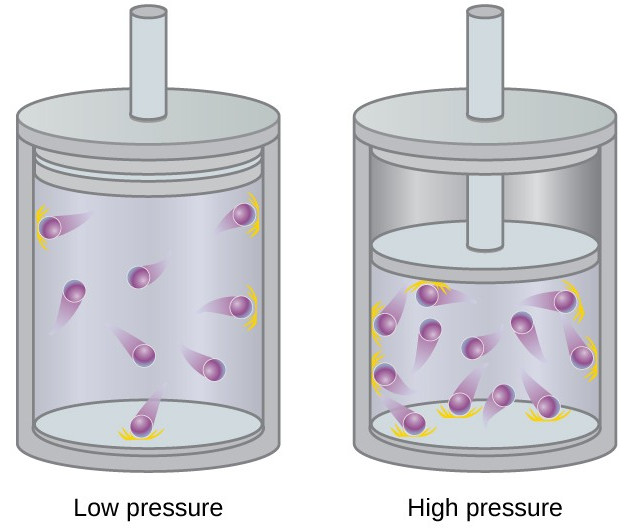
\includegraphics[width=\linewidth]{idealgas.jpg}

\column{0.6\linewidth}
\Large
It's an abstraction like thermodynamics; it can be exact with the right definitions.
\end{columns}
\end{uncoverenv}
\end{frame}

\begin{frame}[fragile]{Most of computer science is about abstracting details, too.}
\scriptsize
\vspace{0.05 cm}
\begin{minted}{c++}
double bessel_j0(double x) {
    double out;
    if (fabs(x) < 8.0) {
        double y = x*x;
        double ans1 = 57568490574.0 + y*(-13362590354.0 + y*(651619640.7
                      + y*(-11214424.18 + y*(77392.33017 + y*(-184.9052456)))));
        double ans2 = 57568490411.0 + y*(1029532985.0 + y*(9494680.718
                      + y*(59272.64853 + y*(267.8532712 + y*1.0))));
        out = ans1 / ans2;
    }
    else {
        double z = 8.0 / fabs(x);
        double y = z*z;
        double xx = fabs(x) - 0.785398164;
        double ans1 = 1.0 + y*(-0.1098628627e-2 + y*(0.2734510407e-4
                      + y*(-0.2073370639e-5 + y*0.2093887211e-6)));
        double ans2 = -0.1562499995e-1 + y*(0.1430488765e-3
                      + y*(-0.6911147651e-5 + y*(0.7621095161e-6
                      - y*0.934935152e-7)));
        out = sqrt(0.636619772/fabs(x))*(cos(xx)*ans1 - z*sin(xx)*ans2);
    }
    return out;
}
\end{minted}

\vspace{-7.95 cm}\hspace{6 cm}{\uncover<2->{\LARGE $\leftarrow$ one value goes in}}

\vspace{6.4 cm}\hspace{6 cm}{\uncover<3->{\LARGE $\leftarrow$ one value comes out}}

\end{frame}

\begin{frame}{}
\Large
\vspace{0.97 cm}
\begin{columns}
\column{0.5\linewidth}
\mbox{\hspace{-3.5 cm}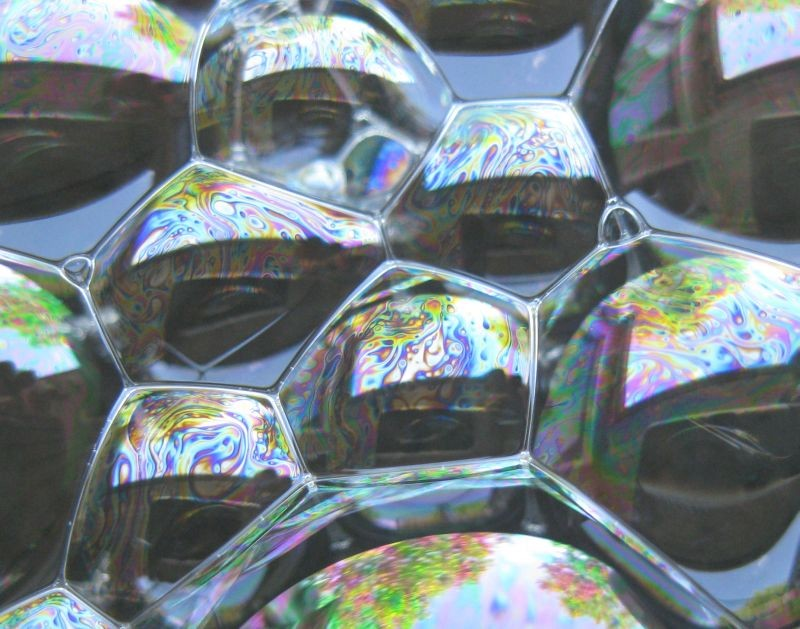
\includegraphics[height=8 cm]{soap-bubbles.jpg}}

\column{0.55\linewidth}
\textcolor{darkblue}{The abstraction is cumulative:}

\vspace{0.25 cm}
Every function/class/module has an interior and an interface---minimizing

\[ \frac{\mbox{\#external parameters}}{\mbox{\#internal parameters}} \]

\vspace{0.25 cm}
reduces the mental burden on programmers and users.
\end{columns}
\end{frame}

\begin{frame}{Science has layers of abstraction}
\large
\vspace{0.75 cm}
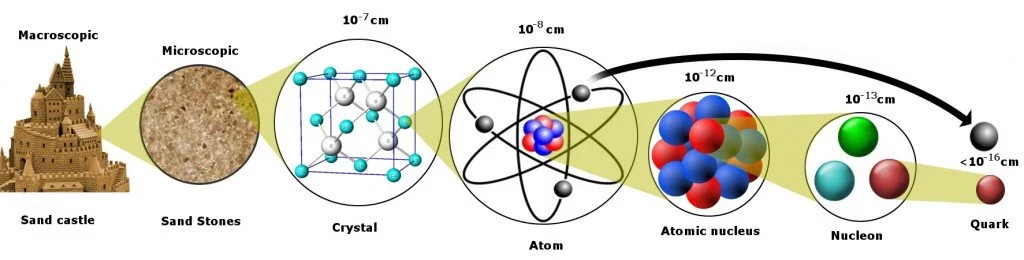
\includegraphics[width=\linewidth]{atom-proton-quark.png}

\vspace{1 cm}
\textcolor{gray}{though these are approximate, taking advantage of a separation of scales.}
\end{frame}

\begin{frame}{(cartoon diagram, not to scale)}
\vspace{0.2 cm}
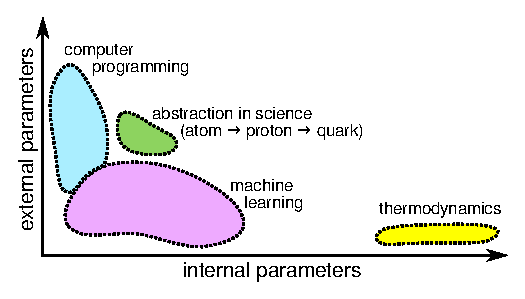
\includegraphics[width=\linewidth]{internal-vs-external.pdf}
\end{frame}

\begin{frame}{Software interfaces can be exact, despite radical internal differences.}
\large
\vspace{0.13 cm}
\begin{itemize}
\item Super Mario Bros.\ \textcolor{darkblue}{entirely rewritten in Javascript} by Josh Goldberg.
\item Shares none of the original code, but behaves identically.
\end{itemize}

\begin{center}
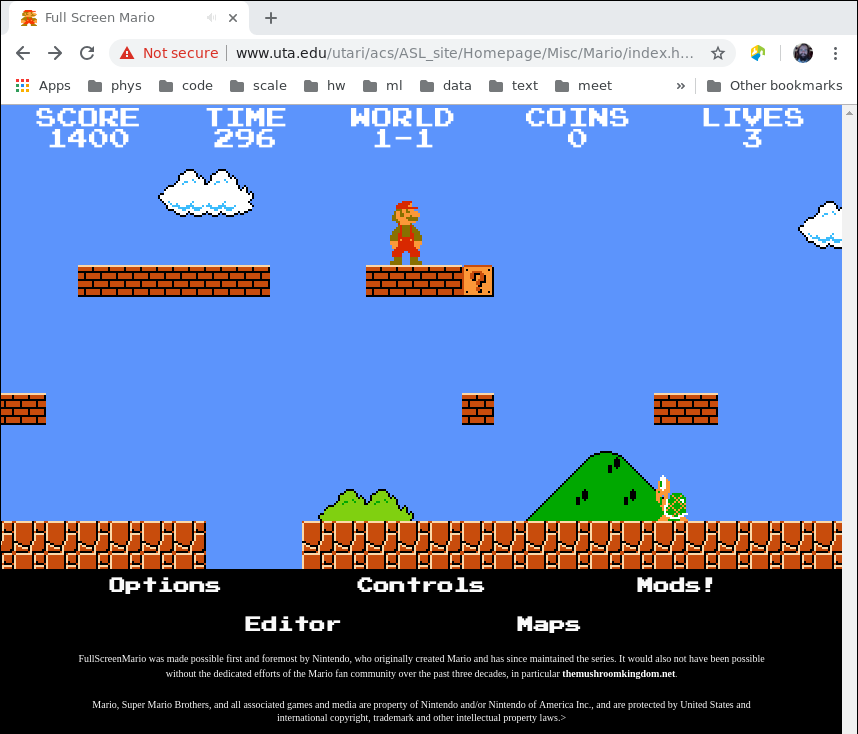
\includegraphics[width=0.97\linewidth]{supermario-javascript.png}
\end{center}

\vspace{-1.8 cm}\mbox{ }\hfill\uncover<2->{\textcolor{yellow}{\bf\huge Is it the same program?}}\hfill\mbox{ }

\vspace{1.8 cm}
\end{frame}

\begin{frame}{}
\vspace{1.25 cm}
\Large
\begin{columns}
\column{0.65\linewidth}
\begin{center}
As a young programmer, I wasn't satisfied with high-level languages because I wanted to get down to the ``real'' computer.

\vspace{0.75 cm}
\uncover<2->{Which meant Pascal. \\ Pascal was ``real,'' and BASIC was not.}

\vspace{0.75 cm}
\uncover<3->{But ultimately, not even assembly code is real in the sense that I meant.}
\end{center}
\column{0.35\linewidth}
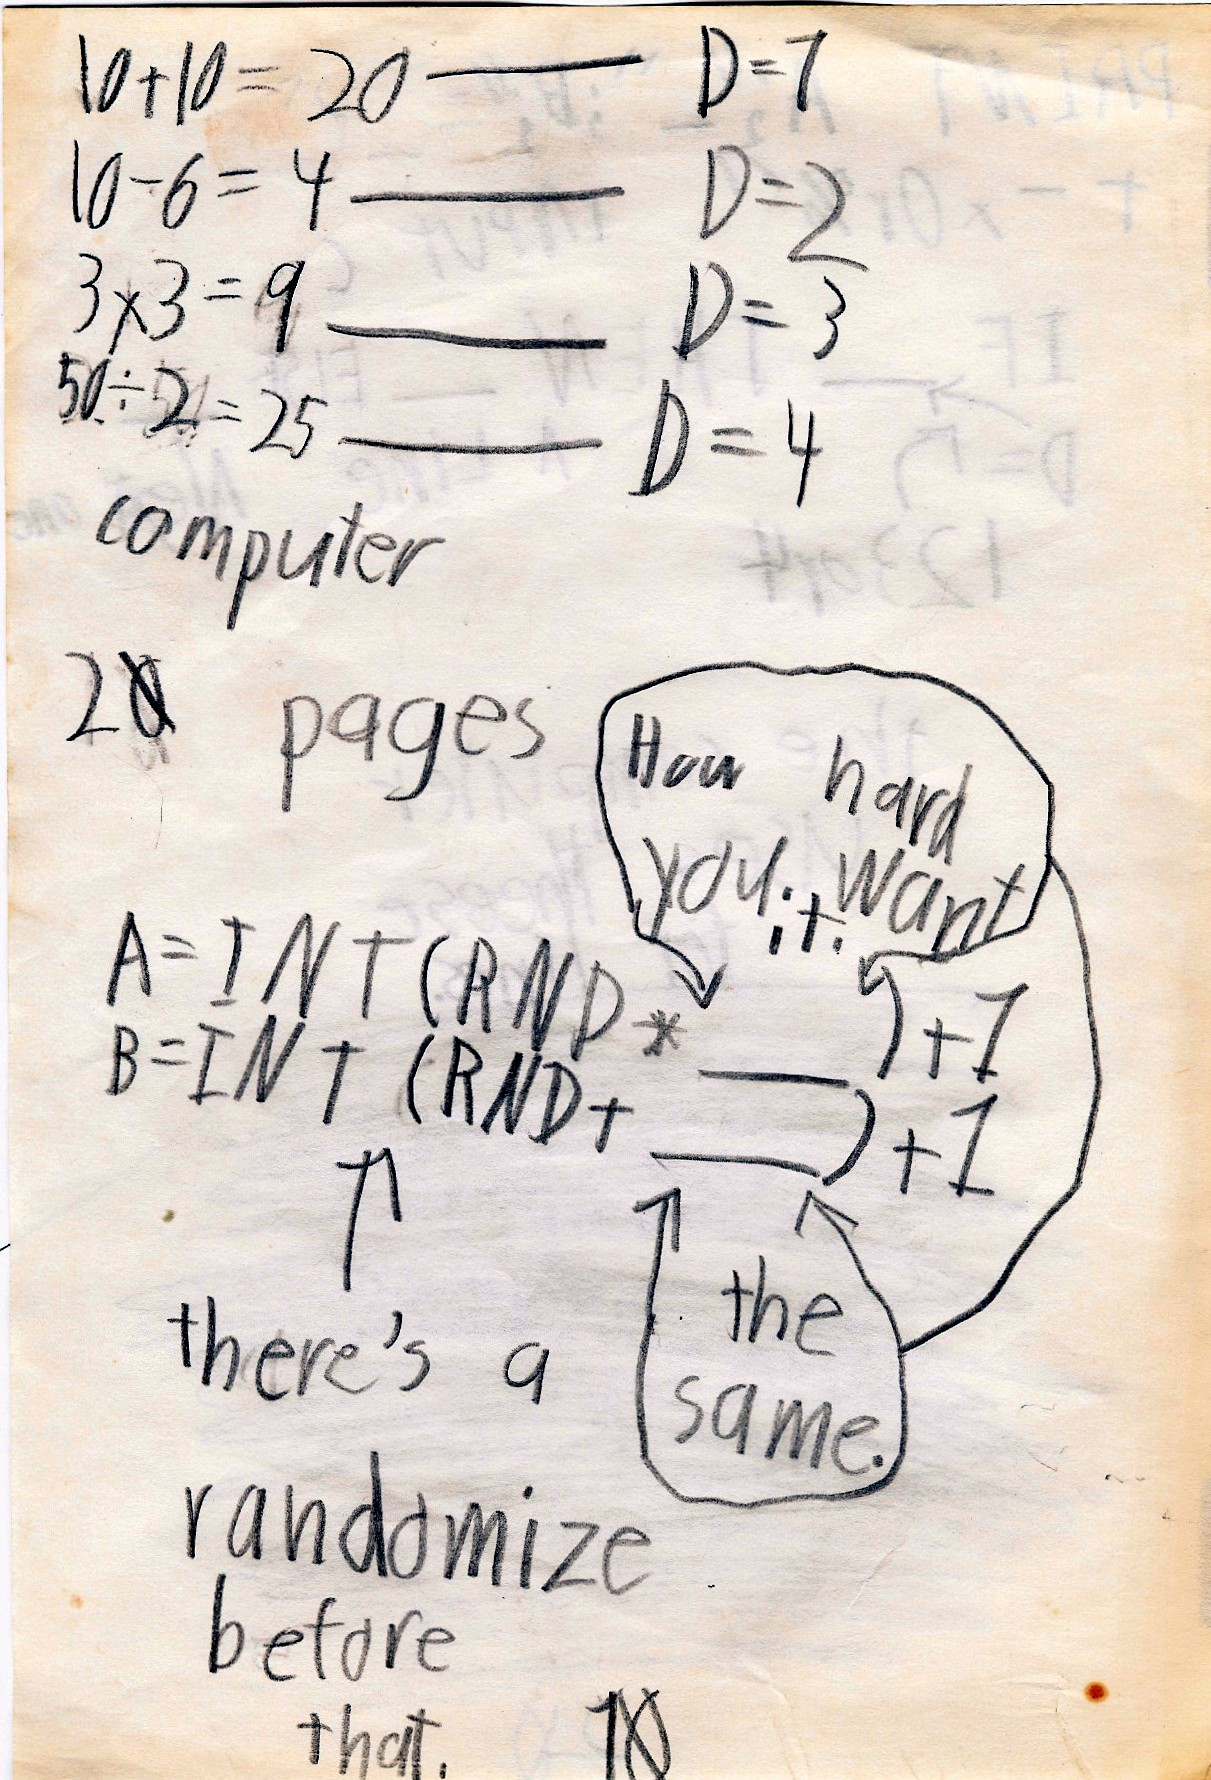
\includegraphics[width=\linewidth]{jimbasic1.jpg}
\end{columns}
\end{frame}

\begin{frame}{}
\LARGE
\vspace{1 cm}
\begin{center}
The objectively real part of a computer is the set of physical states \underline{\it that we interpret} as computations.

\vspace{0.2 cm}
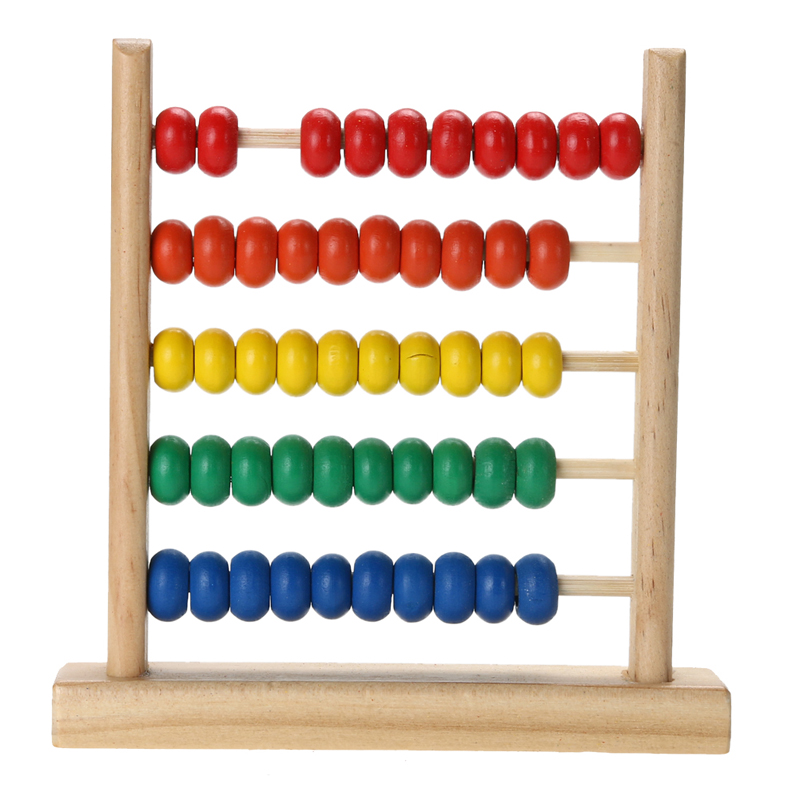
\includegraphics[width=0.4\linewidth]{abacus.jpg}
\end{center}
\end{frame}

\begin{frame}{Programming languages are how we \underline{\it describe} our interpretations.}
\Large
\vspace{0.75 cm}
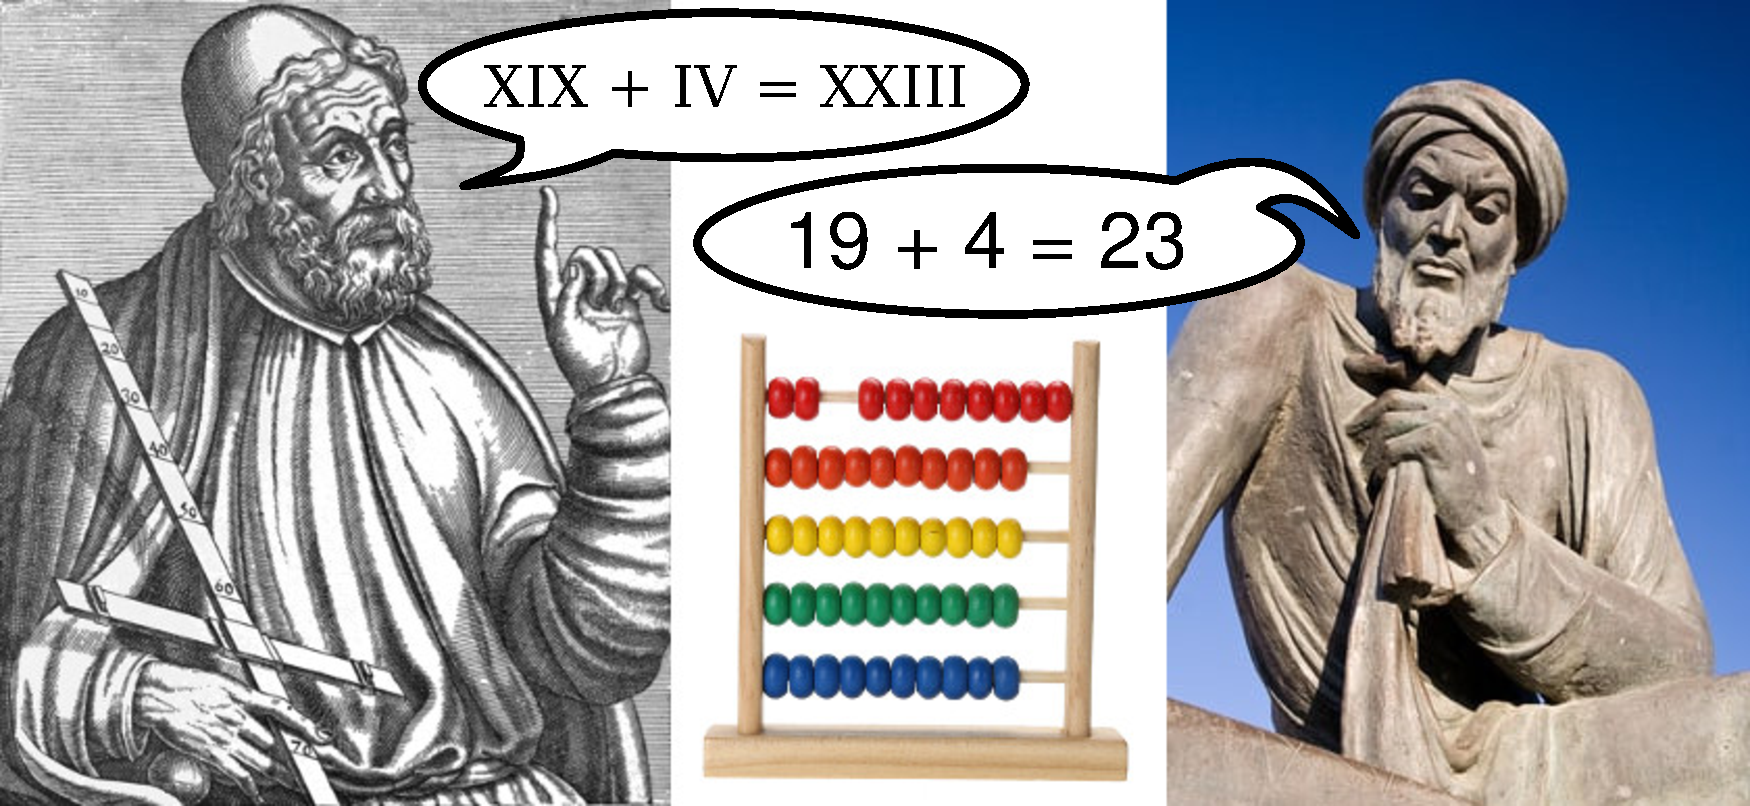
\includegraphics[width=\linewidth]{abacus_ptolemy_al-khwarizmi.pdf}

\vspace{-0.2 cm}
\begin{center}
\uncover<2->{(And some languages are better at it than others.)}
\end{center}
\end{frame}

\begin{frame}{}
\Large
\vspace{1.25 cm}
\begin{center}
Programming languages differ in their degree of abstraction, \\
but {\it all} programming languages are for humans, not computers.

\vspace{0.75 cm}
\begin{uncoverenv}<2->
Each one re-expresses the programmer's intent in terms of another:

\large
\vspace{0.25 cm}
\begin{tabular}{r c l}
CMSSW configuration & \textcolor{darkblue}{implemented in} & Python runtime \\
Python runtime & \textcolor{darkblue}{implemented in} & C source code \\
C source code & \textcolor{darkblue}{compiled into} & machine instructions \\
machine instructions & \textcolor{darkblue}{built into} & logic gates \\
logic gates & \textcolor{darkblue}{interpreted as} & computation.
\end{tabular}
\end{uncoverenv}

\vspace{0.75 cm}
\uncover<3->{\Large Only the last level actually pushes the abacus beads.}
\end{center}
\end{frame}

\begin{frame}{Originally, programming languages {\it didn't} push the abacus beads.}
\vspace{0.25 cm}
\begin{columns}
\column{0.5\linewidth}
\textcolor{darkblue}{Ada of Lovelace's} algorithm for computing Bernoulli numbers was written for a computer that never ended up being invented, but it was a program.

\column{0.5\linewidth}
\hfill\mbox{\hspace{-1 cm}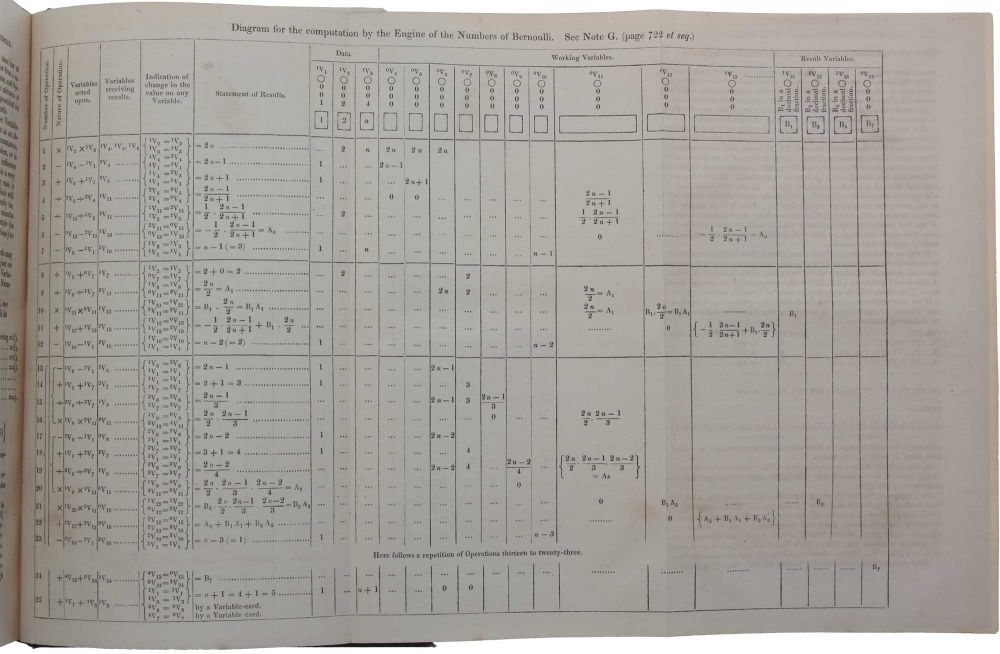
\includegraphics[height=3 cm]{ada-program.jpg}\hspace{0.5 cm}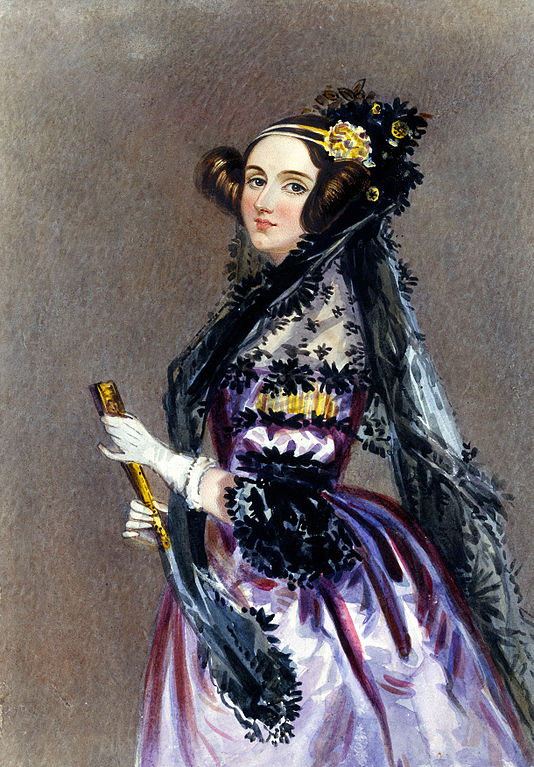
\includegraphics[height=3 cm]{ada.jpg}}
\end{columns}

\vspace{0.5 cm}
\begin{uncoverenv}<2->
\begin{columns}
\column{1.05\linewidth}
\textcolor{darkblue}{John McCarthy, creator of Lisp:} ``This EVAL was written and published in the paper and Steve Russel said, `Look, why don't I program this EVAL?' and I said to him, `Ho, ho, you're confusing theory with practice---this EVAL is intended for reading, not for computing!' But he went ahead and did it.''
\end{columns}
\end{uncoverenv}

\vspace{0.5 cm}
\begin{uncoverenv}<3->
\begin{columns}
\column{1.05\linewidth}
\textcolor{darkblue}{APL (ancestor of MATLAB, R, and Numpy)} was also a notation for describing programs years before it was executable. The book was named {\it A Programming Language}.
\end{columns}
\end{uncoverenv}
\end{frame}

\begin{frame}{}
\Large
\vspace{1.25 cm}
\begin{center}
Programmers had to manually translate \\ these notations into instruction codes.

\vspace{1 cm}
{\huge That's why it was called ``coding.''}

\vspace{1 cm}
\uncover<2->{Von Neumann called assembly language ``\textcolor{darkblue}{a waste of a valuable scientific computing instrument---using it for clerical work!}''}
\end{center}
\end{frame}

\begin{frame}{The Software Crisis}
\large
\vspace{1 cm}
Now that our programming languages {\it do} push abacus beads, software engineering has become an odd discipline: \textcolor{darkblue}{describing something is the same as creating it.}

\vspace{1 cm}
\begin{uncoverenv}<2->
And yet, we {\it still} get it wrong.

\vspace{0.25 cm}
\begin{center}

\includegraphics[width=0.6\linewidth]{literal-genie.png}
\end{center}
\end{uncoverenv}
\end{frame}

\begin{frame}{}
\Large
\vspace{1.5 cm}
\begin{columns}
\column{1.03\linewidth}
\begin{center}
We favor \textcolor{darkblue}{high-level} languages because they have fewer concepts, hopefully just the ones that are essential for a problem.

\vspace{1 cm}
\uncover<2->{\textcolor{darkorange}{\bf But what about speed?} Don't we choose languages for speed?}

\vspace{1 cm}
\begin{uncoverenv}<3->
``There's no such thing as a `fast' or `slow' language.''

\vspace{0.2 cm}
\hfill\mbox{--- StackOverflow\hspace{1 cm}}
\end{uncoverenv}
\end{center}
\end{columns}
\end{frame}

\begin{frame}{Except Python. Python is slow, right?}
\vspace{0.25 cm}
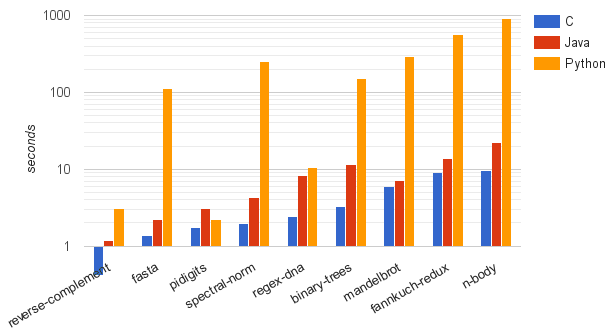
\includegraphics[width=\linewidth]{benchmark-games.png}

\vspace{-0.5 cm}
\mbox{ }\hfill\textcolor{blue}{\tiny \url{https://benchmarksgame-team.pages.debian.net/benchmarksgame}}\hfill\mbox{ }
\end{frame}

\begin{frame}[fragile]{But it really isn't the language; it's the implementation.}
\vspace{0.5 cm}
\hfill\mbox{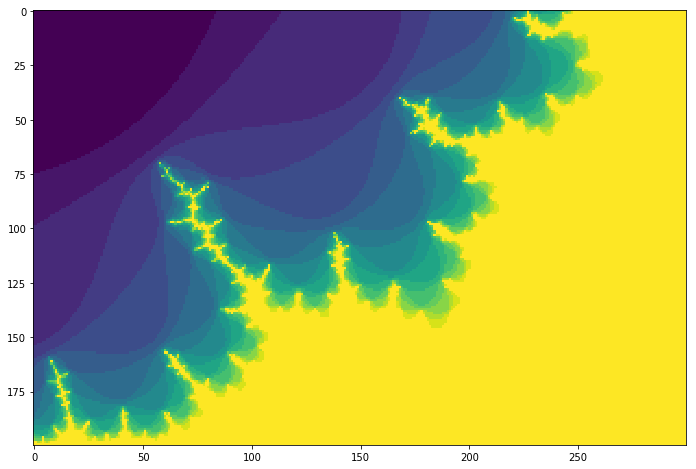
\includegraphics[height=3 cm]{performance-test-fractal.png}\hspace{-0.25 cm}}

\vspace{-2.5 cm}
\scriptsize
\begin{columns}
\column{1.08\linewidth}
\begin{onlyenv}<1>
\begin{minted}{python}
import numpy

def run(height, width, maxiterations=20):
    y, x = numpy.ogrid[-1:0:height*1j, -1.5:0:width*1j]
    c = x + y*1j
    fractal = numpy.full(c.shape, maxiterations,
                                  dtype=numpy.int32)
    for h in range(height):
        for w in range(width):                  # for each pixel (h, w)...
            z = c[h, w]
            for i in range(maxiterations):      # iterate at most 20 times
                z = z**2 + c[h, w]              # applying z → z² + c
                if abs(z) > 2:                  # if it diverges (|z| > 2)
                    fractal[h, w] = i           # color the plane with the iteration number
                    break                       # we're done, no need to keep iterating

    return fractal
\end{minted}
\end{onlyenv}
\begin{onlyenv}<2>
\begin{minted}{python}
import numpy, numba
@numba.jit
def run(height, width, maxiterations=20):
    y, x = numpy.ogrid[-1:0:height*1j, -1.5:0:width*1j]
    c = x + y*1j
    fractal = numpy.full(c.shape, maxiterations,
                                  dtype=numpy.int32)
    for h in range(height):
        for w in range(width):                  # for each pixel (h, w)...
            z = c[h, w]
            for i in range(maxiterations):      # iterate at most 20 times
                z = z**2 + c[h, w]              # applying z → z² + c
                if abs(z) > 2:                  # if it diverges (|z| > 2)
                    fractal[h, w] = i           # color the plane with the iteration number
                    break                       # we're done, no need to keep iterating

    return fractal
\end{minted}
\end{onlyenv}
\end{columns}

\large
\vspace{0.25 cm}
\begin{center}
\uncover<2->{Now \textcolor{darkorange}{\bf 50$\times$ faster}, about equal to C code ({\tt -O3}).}
\end{center}
\end{frame}

\begin{frame}{Here's the catch}
\large
\vspace{0.5 cm}
The \mintinline{python}{@numba.jit} decorator translates {\it a subset of} Python bytecode to machine instructions. You only get a speedup for statically typable, numeric code.

\begin{center}
\Large \uncover<2->{Same language, completely different implementation.}
\end{center}

\begin{uncoverenv}<3->
\begin{center}
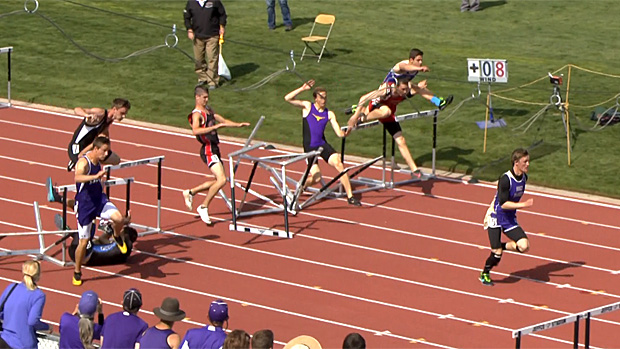
\includegraphics[width=0.4\linewidth]{hurdle9.jpg}
\end{center}

Python is slower than Numba or C because it has more hurdles in the way: dynamic typing, pointer-chasing, garbage collection, hashtables, string equality\ldots
\end{uncoverenv}
\end{frame}

\begin{frame}{Greg Owen's talk on Spark 2.0}
\vspace{0.17 cm}
\begin{center}
\only<1>{
\includegraphics[width=0.95\linewidth]{greg-owen/page1.png}}\only<2>{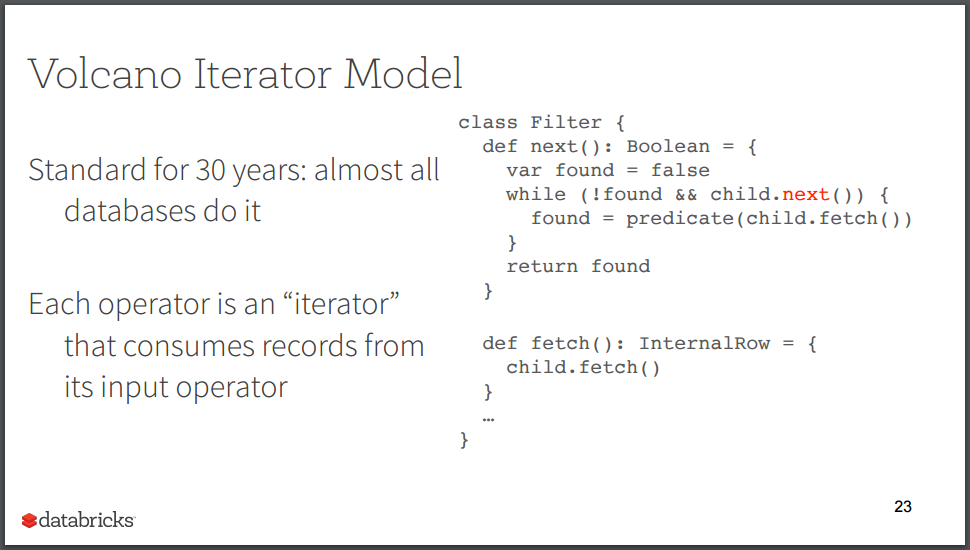
\includegraphics[width=0.95\linewidth]{greg-owen/page2.png}}\only<3>{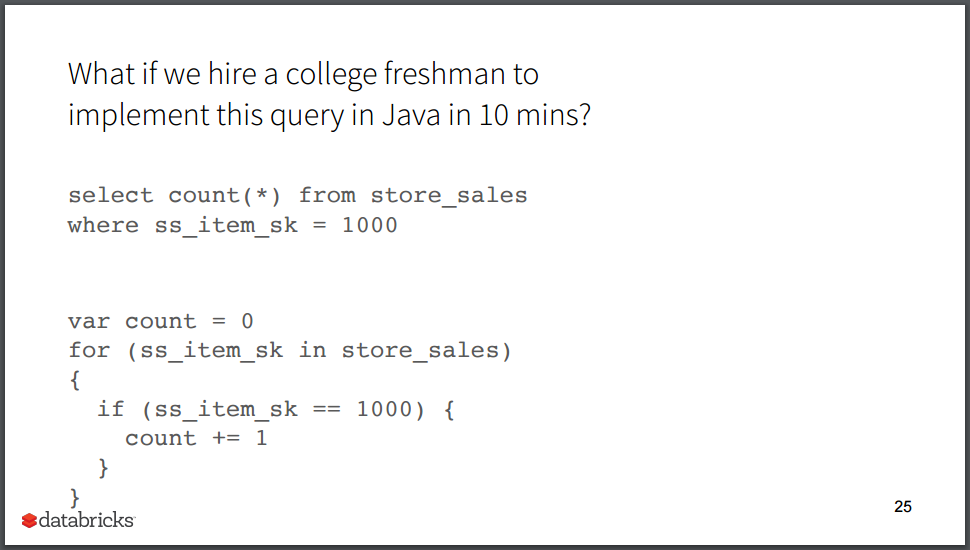
\includegraphics[width=0.95\linewidth]{greg-owen/page3.png}}\only<4>{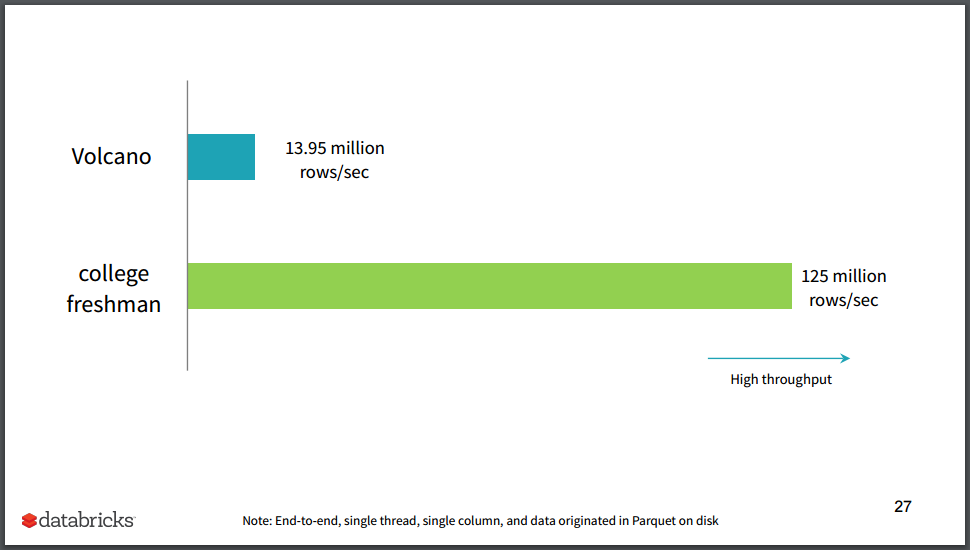
\includegraphics[width=0.95\linewidth]{greg-owen/page4.png}}\only<5>{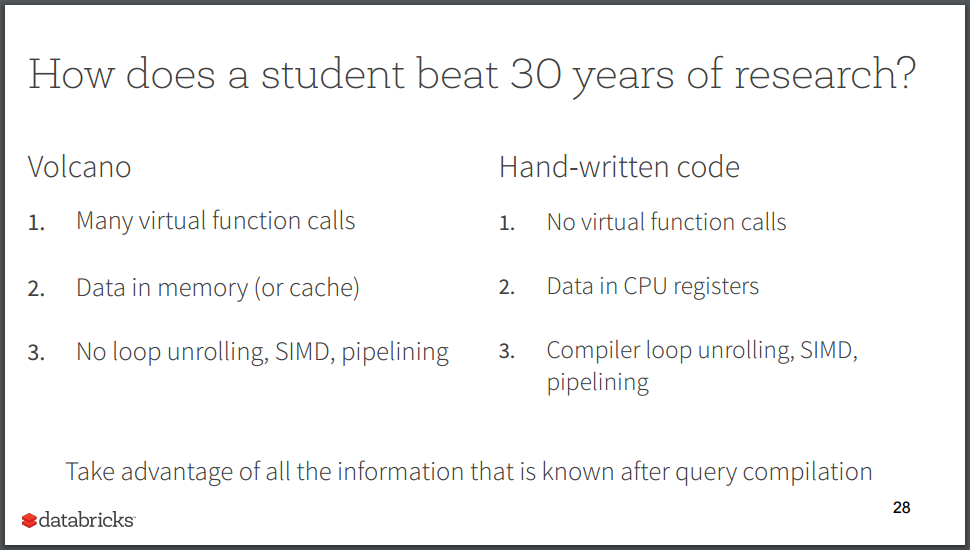
\includegraphics[width=0.95\linewidth]{greg-owen/page5.png}}
\end{center}
\end{frame}

\begin{frame}{}
\Large
\vspace{1 cm}
\begin{center}
So although it's the implementation, not the language, that's slow,

\vspace{1 cm}
that implementation can be hampered by the flexibility \\ that the language promises.
\end{center}
\end{frame}

\begin{frame}{}
\begin{columns}[t]
\column{1.16\linewidth}
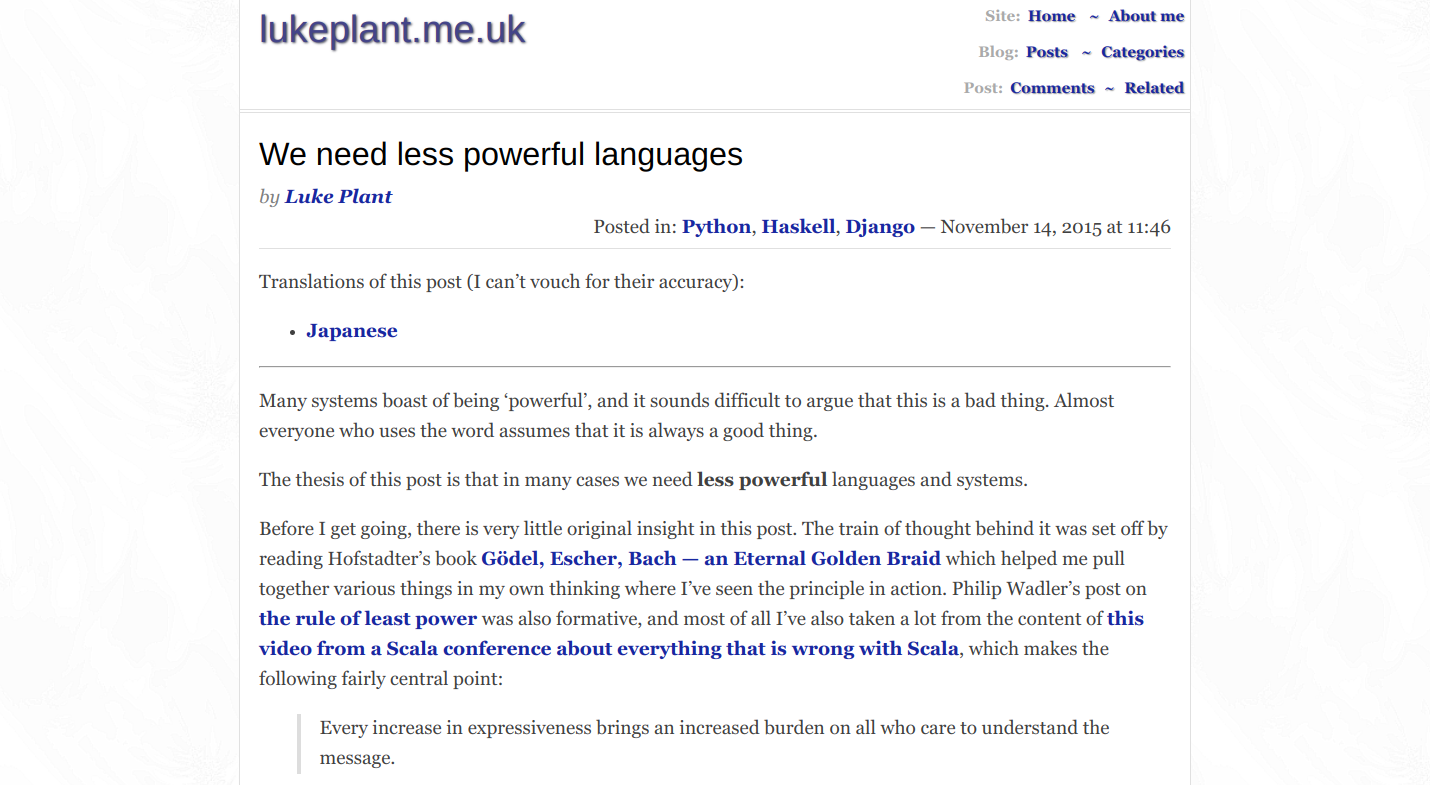
\includegraphics[width=\linewidth]{less-powerful.png}
\end{columns}
\end{frame}

\begin{frame}{}
\LARGE
\vspace{1.25 cm}
\textcolor{darkblue}{Domain-specific languages:}

\vspace{0.5 cm}
\Large
\begin{columns}
\column{0.85\linewidth}
specialized languages for narrowly defined problems.

\large
\vspace{0.5 cm}
\begin{itemize}\setlength{\itemsep}{0.5 cm}
\item \textcolor{darkblue}{Main purpose:} reduces complexity, the mental clutter that obscures general-purpose languages.
\item \textcolor{darkblue}{Secondary purpose:} limited flexibility allows for streamlined implementations.
\end{itemize}
\end{columns}
\end{frame}

\begin{frame}{Domain-specific languages that you're probably already using}
\huge
\vspace{1 cm}
\begin{center}
Any guesses?
\end{center}
\end{frame}

\begin{frame}{Domain-specific languages that you're probably already using}
\LARGE
\vspace{0.25 cm}

\textcolor{darkblue}{Regular expressions}

\begin{center}
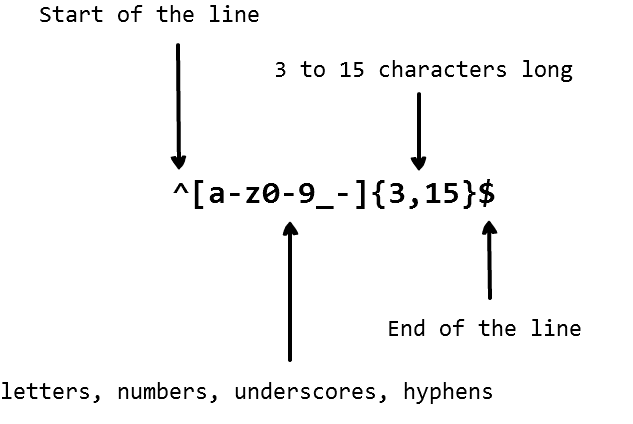
\includegraphics[width=0.7\linewidth]{regex.png}
\end{center}
\end{frame}

\begin{frame}[fragile]{Domain-specific languages that you're probably already using}
\LARGE
\vspace{0.5 cm}

\textcolor{darkblue}{TTree::Draw (TTreeFormula)}

\vspace{-1 cm}
\normalsize
\begin{columns}
\column{0.61\linewidth}
\begin{minted}{c++}
ttree->Draw("lep1_p4.X() + lep1_p4.Y()");
\end{minted}

\column{0.3\linewidth}
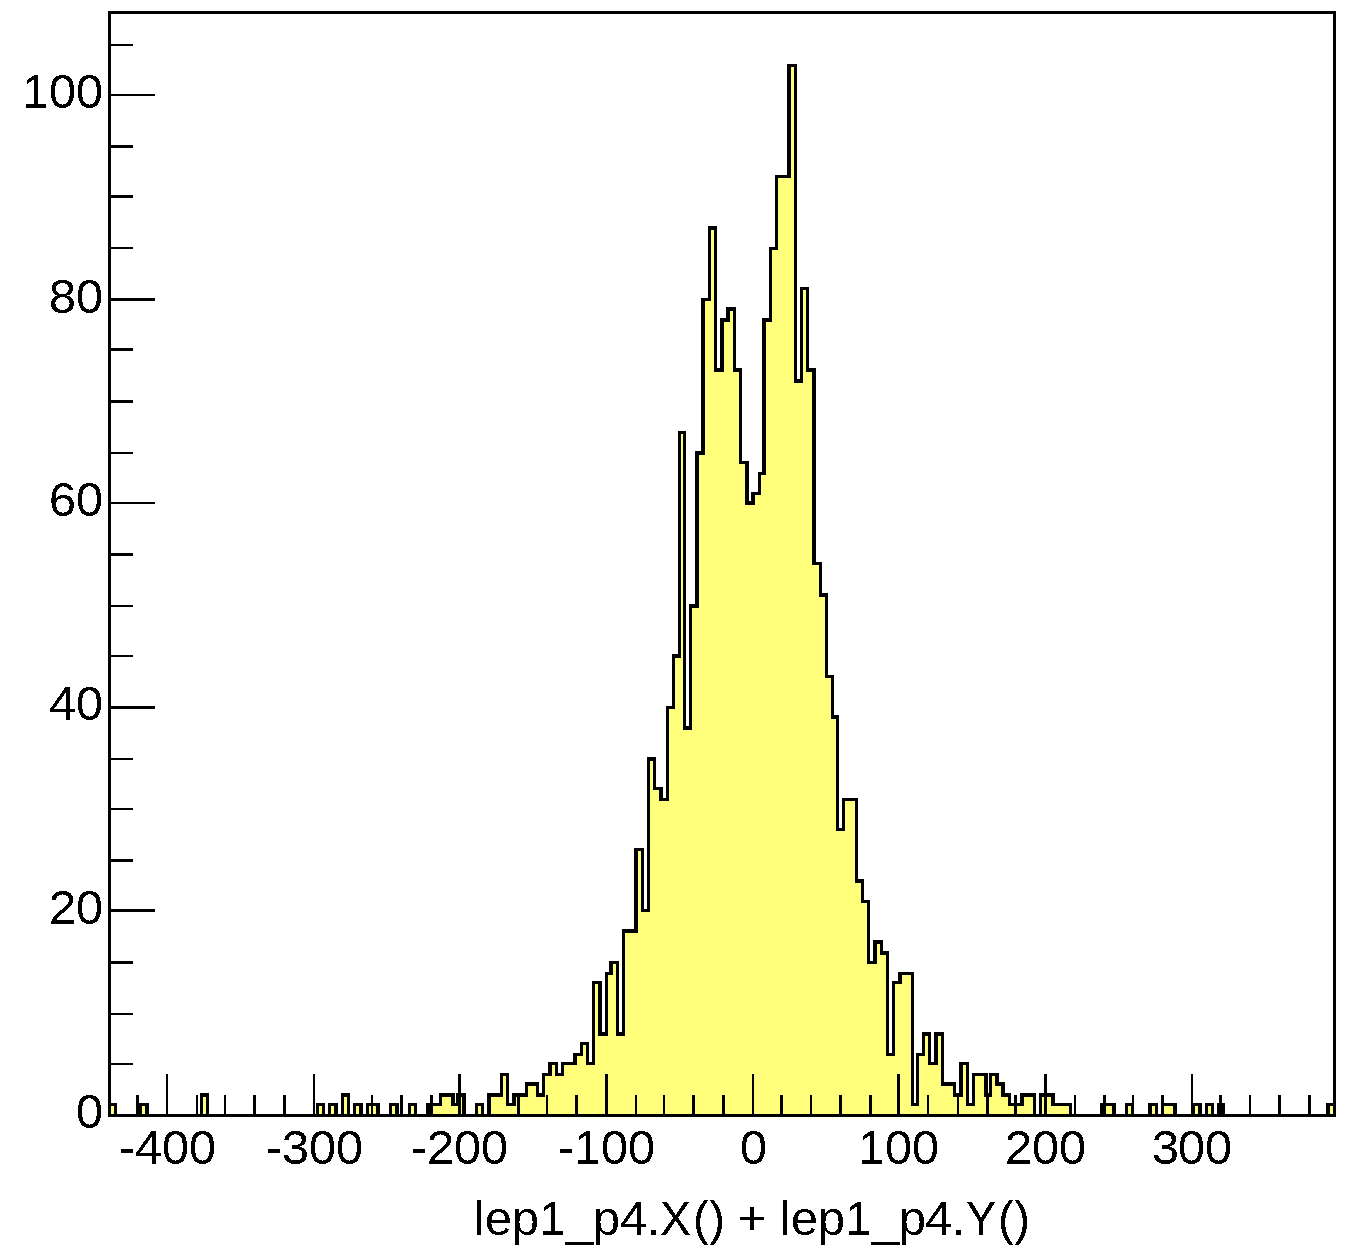
\includegraphics[width=\linewidth]{ttree-draw.pdf}
\end{columns}

\vspace{-0.5 cm}
\begin{uncoverenv}<2->
\textcolor{darkblue}{\large Looping and reducing constructs:}

\vspace{0.25 cm}
\begin{columns}
\column{0.35\linewidth}
\mintinline{c++}{"fMatrix[][fResults[][]]"}

\column{0.02\linewidth}
\mbox{\hspace{0.5 cm}$\longrightarrow$}

\column{0.5\linewidth}
\scriptsize
\begin{minted}{c++}
for (int i0; i0 < 3; i0++) {
   for (int j2; j2 < 5; j2++) {
      for (int j3; j3 < 2; j3++) {
         int i1 = fResults[j2][j3];
         use the value of fMatrix[i0][i1]
   }
}
\end{minted}
\end{columns}

\vspace{0.5 cm}
\mbox{\tt\small Length\$($\cdot$) Sum\$($\cdot$) Min\$($\cdot$) Max\$($\cdot$) MinIf\$($\cdot$,$\cdot$) MaxIf\$($\cdot$,$\cdot$) Alt\$($\cdot$,$\cdot$)\hspace{1 cm}}
\end{uncoverenv}
\end{frame}

\begin{frame}{Domain-specific languages that you're probably already using}
\LARGE
\vspace{0.25 cm}

\textcolor{darkblue}{Makefiles}

\vspace{0.25 cm}
\begin{center}
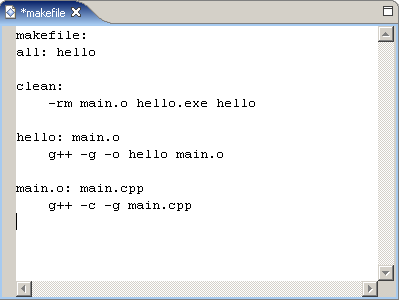
\includegraphics[width=0.5\linewidth]{makefile.png}
\end{center}
\end{frame}

\begin{frame}[fragile]{Domain-specific languages that you're probably already using}
\LARGE
\vspace{0.25 cm}

\textcolor{darkblue}{Format strings}

\vspace{0.5 cm}
{\large \textcolor{darkblue}{printf/scanf:} distinct syntax from C/C++, must be quoted}

\small
\begin{minted}{c++}
printf("Error 0x%04x: %s", id, errors[id]);
\end{minted}

\vspace{0.5 cm}
{\large \textcolor{darkblue}{I/O streams:} defined within C/C++ via operator overloading}

\small
\begin{minted}{c++}
std::cout << "Error 0x" << std::hex << std::setfill('0')
          << std::setw(4) << id << ": " << errors[id] << std::endl;
\end{minted}

\large
\vspace{0.05 cm}
\begin{center}
\uncover<2->{\textcolor{darkblue}{printf/scanf} is ``external'' and \textcolor{darkblue}{I/O streams} is ``internal'' (embedded)}
\end{center}
\end{frame}

\begin{frame}[fragile]{External versus internal (embedded) domain-specific languages}
\vspace{0.3 cm}

{\large \textcolor{darkblue}{\underline{External}:} SQL has a distinct syntax from Python; must be quoted in PySpark.}

\small
\vspace{-0.25 cm}
\begin{columns}
\column{0.85\linewidth}
\begin{minted}{python}
import pyspark
pyspark.sql("""
    SELECT CONCAT(first, " ", last) AS fullname, AVG(age)
        FROM my_table WHERE age BETWEEN 18 AND 24
        GROUP BY fullname
""")
\end{minted}
\end{columns}

\vspace{0.5 cm}
{\large \textcolor{darkblue}{\underline{Internal} (embedded):} SparkSQL is an equivalent language, defined within Python.}

\small
\vspace{-0.25 cm}
\begin{columns}
\column{0.85\linewidth}
\begin{minted}{python}
import pyspark.sql.functions as F
df = pyspark.read.load("my_table")
(df.withColumn("fullname",
        F.concat(F.col("first"), F.lit(" "), F.col("last")))
   .select("fullname", "age")
   .where(df.age.between(18, 24))
   .groupBy("fullname")
   .agg(F.mean("age")))
\end{minted}
\end{columns}
\end{frame}

\begin{frame}{}
\large
\vspace{1.5 cm}
\textcolor{darkblue}{\Large Objection:} a collection of libraries and operator overloads isn't a language!

\vspace{1 cm}
\begin{uncoverenv}<2->
\begin{columns}
\column{0.87\linewidth}
\textcolor{darkblue}{\Large My answer:} programming languages are human modes of expression, implemented using other programming languages, all the way down.

\vspace{0.35 cm}
What matters is whether it's a coherent set of concepts, not whether it was implemented by a parser.
\end{columns}
\end{uncoverenv}

\vspace{1 cm}
\uncover<3->{(One might as well argue about the distinction between languages and dialects.)}
\end{frame}

\begin{frame}[fragile]{Behold the flexibility of Scala!}
\large
\vspace{0.5 cm}
In Scala, a class's methods can be accessed through a dot or a space.

\vspace{0.25 cm}
Parentheses are optional on single argument methods, and methods can have unicode names.

\vspace{0.25 cm}
The following are equivalent:

\small
\begin{minted}{scala}
a.cross(b)     // a and b are ThreeVectors, which has a cross method
a cross b      // the dot and parentheses may be omitted
a × b          // cross can also be named ×
\end{minted}
\end{frame}

\begin{frame}[fragile]{What you can do with that: ScalaTest}
\vspace{0.25 cm}

\small
\begin{minted}{scala}
def unitTests(x: Double, str: String) {
    f(x) should not equal 7

    List("one", "two", "three") should contain ("two")

    an [IndexOutOfBoundsException] should be thrownBy str.charAt(-1)
}
\end{minted}

\vspace{0.25 cm}
\begin{uncoverenv}<2->
\begin{columns}
\column{1.05\linewidth}
\large
\textcolor{darkblue}{Works because of syntax magic:}

\normalsize
\begin{itemize}
\item Certain types are promoted to implicit classes with \mintinline{scala}{should} methods.
\item The class returned by \mintinline{scala}{should} has \mintinline{scala}{not}, \mintinline{scala}{contain}, and \mintinline{scala}{be} methods.
\item Some are parameterized (like C++ templates) by \mintinline{scala}{IndexOutOfBoundsException}.
\item Evaluation of arguments may be delayed to internally wrap with try-catch logic.
\end{itemize}

\large
\vspace{0.25 cm}
\uncover<3->{\textcolor{darkorange}{\bf We're not thinking about any of that when we read the test code.}}
\end{columns}
\end{uncoverenv}
\end{frame}

\begin{frame}[fragile]{Another example: Chisel, a hardware description language in Scala}
\scriptsize
\vspace{0.5 cm}

\begin{columns}
\column{1.05\linewidth}
\begin{minted}{scala}
class VendingMachine extends Component {
  val io = new Bundle {
    val nickel = Bool(INPUT)
    val dime   = Bool(INPUT)
    val ready  = Bool(OUTPUT)
  }
  val s_idle :: s_5 :: s_10 :: s_15 :: s_ok :: Nil = Enum(5){ UFIx() }
  val state = Reg(resetVal = s_idle)
  switch (state) {
    is (s_idle) { when (io.nickel) { state := s_5 }  when (io.dime) { state := s_10 } }
    is (s_5)    { when (io.nickel) { state := s_10 } when (io.dime) { state := s_15 } }
    is (s_10)   { when (io.nickel) { state := s_15 } when (io.dime) { state := s_ok } }
    is (s_15)   { when (io.nickel) { state := s_ok } when (io.dime) { state := s_ok } }
    is (s_ok)   { state := s_idle }
  }
  io.ready := (state === s_ok)
}
\end{minted}

\large
\vspace{0.25 cm}
\textcolor{gray}{(It's a register-transfer level hardware description language like Verilog and VHDL, not high-level synthesis, but much more succinct and parameterizable.)}
\end{columns}
\end{frame}

\begin{frame}{}
\Large
\vspace{1 cm}
\begin{columns}
\column{1.1\linewidth}
\begin{center}
Perhaps the most widespread domain-specific language in data analysis:

\vspace{0.5 cm}
{\Huge SQL}

\vspace{1 cm}
\uncover<2->{But we rarely use it in particle physics. Why?}
\end{center}
\end{columns}
\end{frame}

\begin{frame}[fragile]{Structure of a collider physics query: \only<1>{C++}\only<2>{SQL}}
\large
\vspace{0.5 cm}
\textcolor{darkblue}{``Momentum of the track with $|\eta|$ $<$ 2.4 that has the most hits.''}

\small
\begin{columns}
\column{0.8\linewidth}
\begin{onlyenv}<1>
\begin{minted}[stripnl=false]{c++}
Track *best = NULL;

for (int i = 0;  i < tracks.size();  i++) {
  if (fabs(tracks[i]->eta) < 2.4)
    if (best == NULL ||
        tracks[i]->hits.size() > best->hits.size())
      best = tracks[i];
}

if (best != NULL)
  return best->pt;
else
  return 0.0;


\end{minted}
\end{onlyenv}
\begin{onlyenv}<2>
\begin{minted}{sql}
WITH hit_stats AS (
  SELECT hit.track_id, COUNT(*) AS hit_count FROM hit
    GROUP BY hit.track_id),
 track_sorted AS (
    SELECT track.*, 
    ROW_NUMBER() OVER (
     PARTITION BY track.event_id
     ORDER BY hit_stats.hit_count DESC)
  track_ordinal FROM track INNER JOIN hit_stats
    ON hit_stats.track_id = track.id
    WHERE ABS(track.eta) < 2.4)
 SELECT * FROM event INNER JOIN track_sorted
   ON track_sorted.event_id = event.id
WHERE
  track_sorted.track_ordinal = 1
\end{minted}
\end{onlyenv}
\end{columns}
\end{frame}

\begin{frame}{}
\large
\vspace{1.25 cm}
The problem is that collisions produce a variable number of particles per event: the tables are ``jagged.''

\vspace{0.75 cm}
\begin{uncoverenv}<2->
This {\it can be} described using SQL's relational concepts:

\begin{itemize}
\item separate tables for events and particles
\item linked by a common ``event number'' index.
\end{itemize}

But each type of particle has to be a separate table and each operation has to be \mintinline{sql}{INNER JOIN}ed to maintain events as objects.
\end{uncoverenv}

\vspace{0.75 cm}
\uncover<3->{SQL makes particle physics problems {\it harder}, not {\it easier}, which defeats the point.}
\end{frame}

\begin{frame}{It seems like there's an opportunity here}
\large
\vspace{0.5 cm}
\textcolor{darkblue}{Would a domain specific language for particle physics}

\begin{itemize}\setlength{\itemsep}{0.25 cm}
\item make analysis code easier to read?
\item make mistakes more evident?
\item make it easier to synchronize analyses from different groups/experiments?
\item make it easier to preserve them in executable/recastable form?
\item highlight physics concepts, like control regions, systematic variations, event weights, combinatorics with symmetries?
\item hide irrelevant concepts like managing files, memory, load balancing, and other performance tweaks?
\end{itemize}

\vspace{0.25 cm}
\uncover<2->{\textcolor{darkorange}{\bf That was the subject of the Analysis Description Language Workshop.}}
\end{frame}

\begin{frame}{}
\LARGE
\vspace{1.25 cm}
\begin{center}
Why hasn't this been done before?

\vspace{1 cm}
\textcolor{gray}{\large (Why hasn't it succeeded before?)}
\end{center}
\end{frame}

\begin{frame}{}
\Large
\vspace{1.25 cm}
\begin{center}
I think the answer is cultural, so I'll take a historical perspective\ldots
\end{center}
\end{frame}

\begin{frame}{The U.S.\ Census's problem}
\large
\vspace{0.35 cm}
The U.S.\ does a census every 10 years. The 1880 census took 8 years to process.
\begin{center}
$\longrightarrow$ Big data problem!
\end{center}

\vspace{0.15 cm}
\begin{uncoverenv}<2->
Held a competition for a new method; winner was 10$\times$ faster than the rest:

\begin{center}
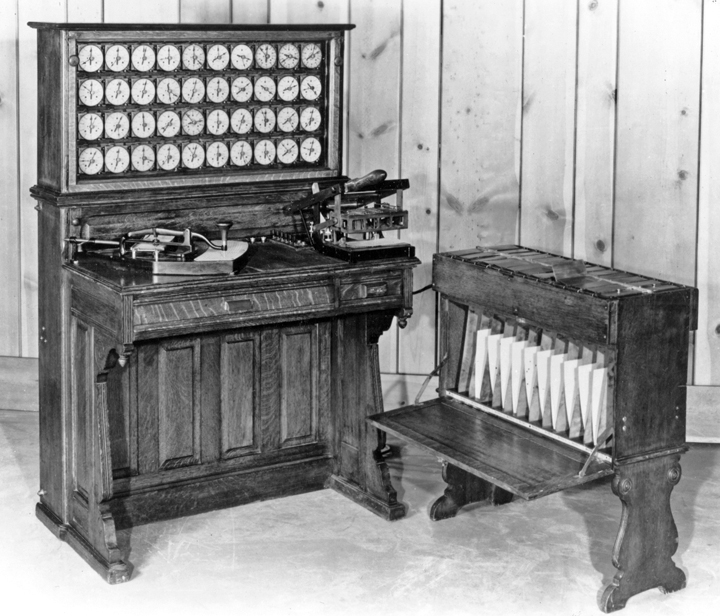
\includegraphics[height=5.3 cm]{hollerith.jpg}\hspace{1 cm}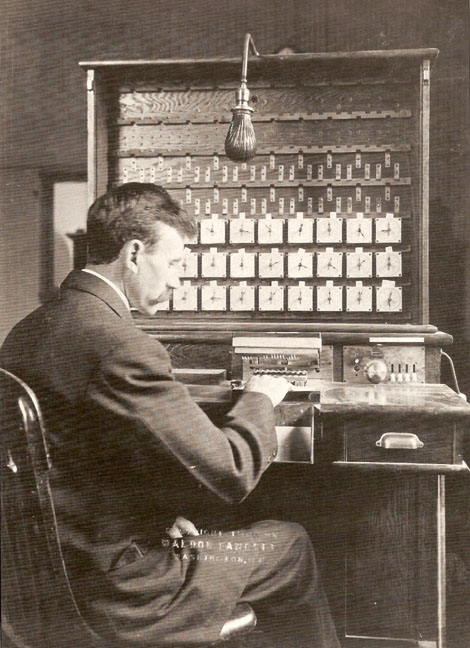
\includegraphics[height=5.3 cm]{1908_Hollerith_Machine.jpg}
\end{center}
\end{uncoverenv}
\end{frame}

\begin{frame}{Census records on punch cards, which filtered electrical contacts}
\vspace{0.17 cm}
\begin{columns}
\column{0.5\linewidth}
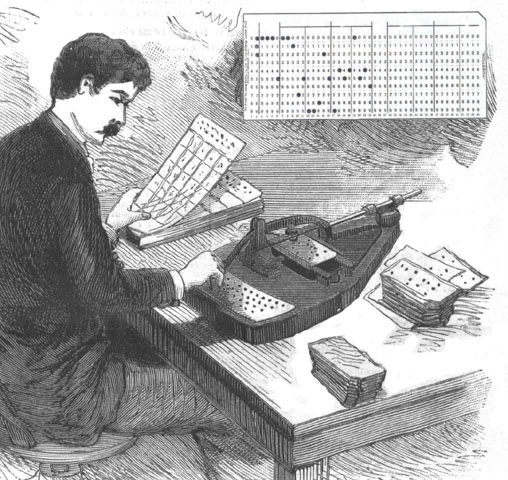
\includegraphics[width=\linewidth]{1890_Census_Hollerith_Pantograph_Punching_Machine_Sci_Amer.jpg}

\column{0.5\linewidth}
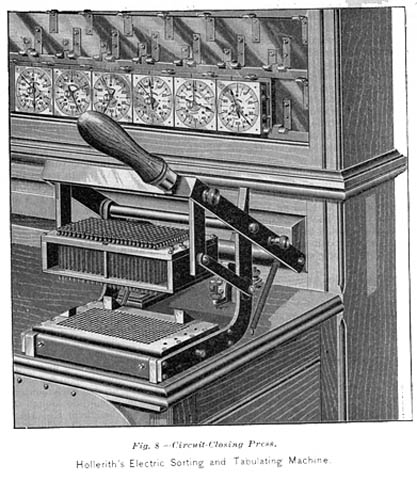
\includegraphics[width=\linewidth]{1890_Hollerith_Circuit-Closing_Press_OM.jpg}
\end{columns}
\end{frame}

\begin{frame}{Wired to a machine that opens a door for each matching pattern}
\vspace{0.25 cm}
\begin{center}
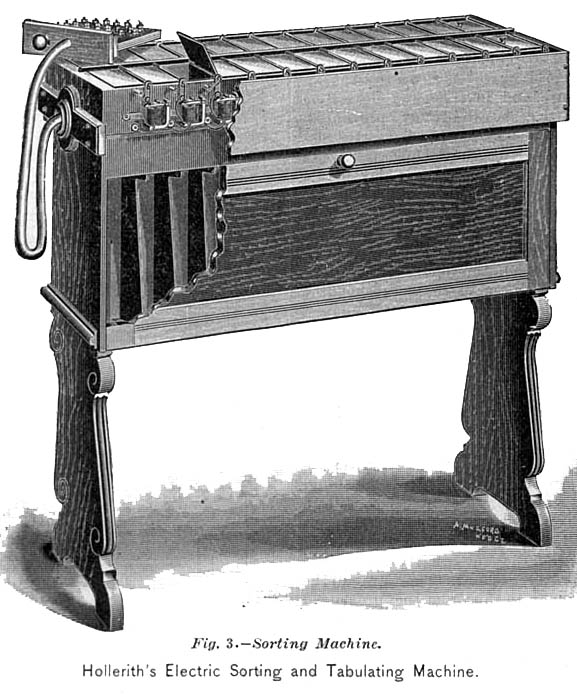
\includegraphics[width=0.45\linewidth]{1890_Hollerith_Sorting_Machine_OM.jpg}
\end{center}
\end{frame}

\begin{frame}{It was an SQL machine: 3 basic clauses of most SQL queries}
\vspace{0.25 cm}
\begin{center}
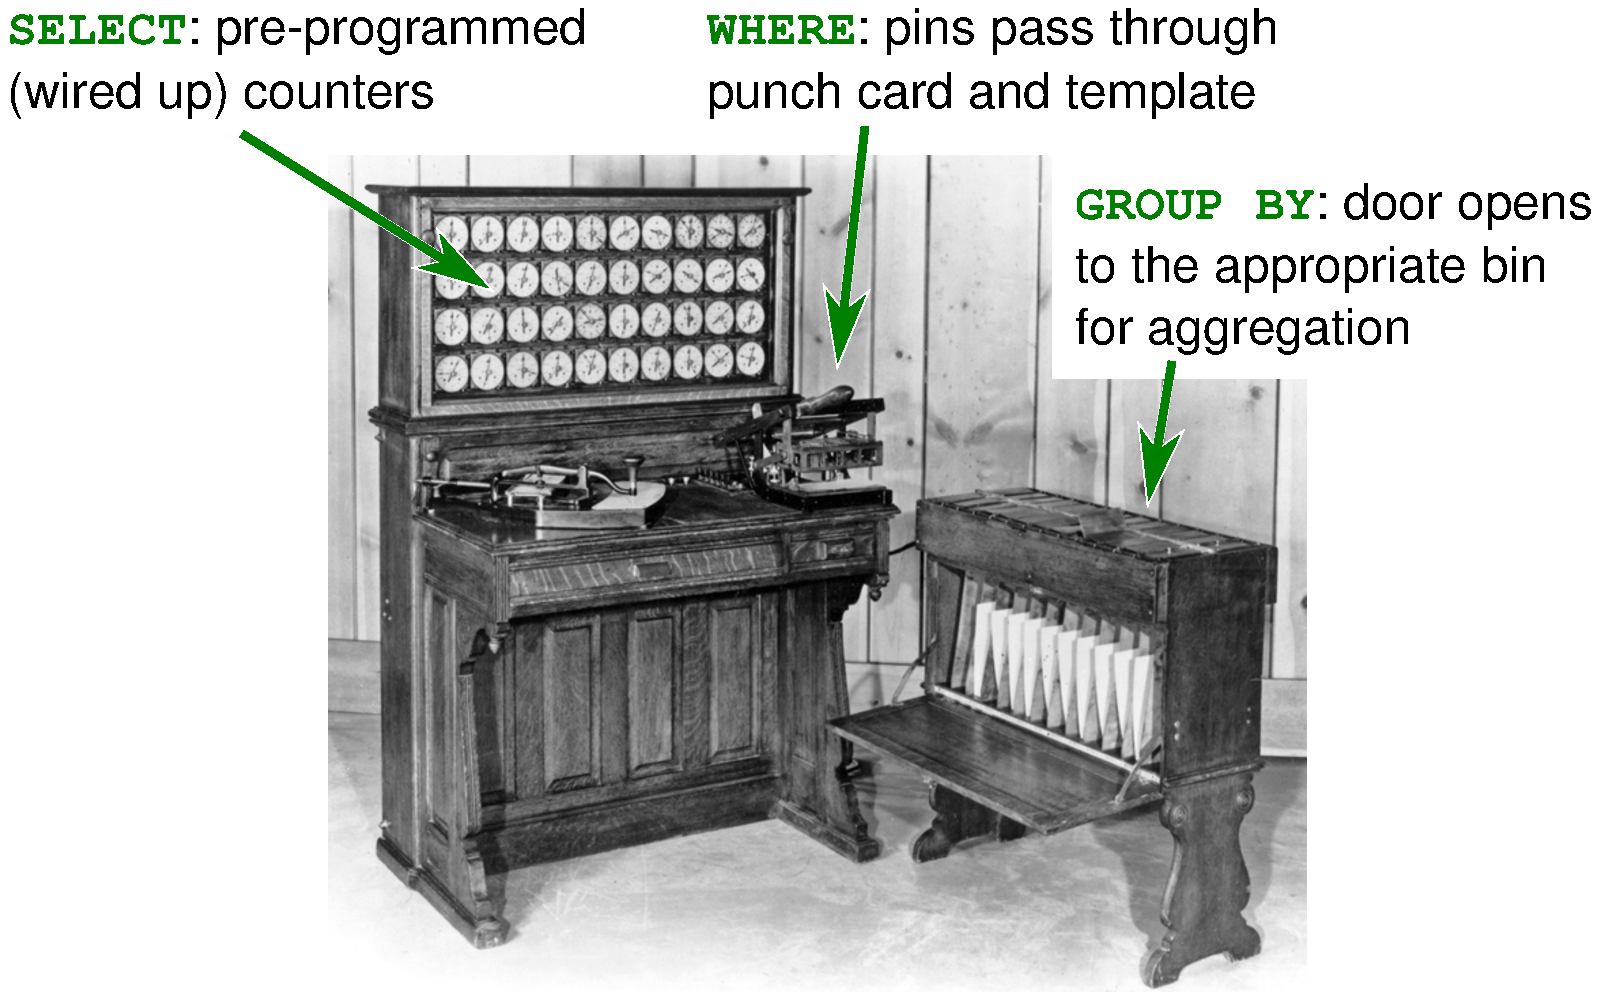
\includegraphics[width=0.75\linewidth]{hh-tabulator.pdf}
\end{center}

\mbox{ } \hfill \mintinline{sql}{SELECT name WHERE literate GROUP BY marital_status} \hfill \mbox{ }
\end{frame}

\begin{frame}{}
\large
\vspace{1.25 cm}
\begin{columns}
\column{1.01\linewidth}
Herman Hollerith (inventor) incorporated the Tabulating Machine Company, which after a series of mergers became International Business Machines (IBM) in 1924.

\vspace{1 cm}
\uncover<2->{The computation represented by this machine is not universal (Turing complete), but has many applications.}

\vspace{0.75 cm}
\begin{center}
\uncover<3->{\textcolor{darkblue}{\LARGE Most recently as ``map-reduce.''}}
\end{center}
\end{columns}
\end{frame}

\begin{frame}{Google's problem}
\large
\vspace{0.45 cm}
In the early 2000's, Google was struggling to keep up with the growing web (index 5 months out of date, routine hardware failures, scale sensitive to bit flips).

\vspace{0.7 cm}
\uncover<2->{Each programmer had to divide tasks and combine results manually, accounting for failures manually.}

\vspace{0.7 cm}
\uncover<3->{2003: MapReduce created to abstract task management from analysis logic.}

\vspace{0.7 cm}
\mbox{ } \hfill \uncover<4->{MapReduce is distributed $\underbrace{\mbox{\mintinline{sql}{SELECT}-\mintinline{sql}{WHERE}}}_{\mbox{``map''}}\mbox{-}\underbrace{\mbox{\mintinline{sql}{GROUP BY}}}_{\mbox{``reduce''}}$.} \hfill \mbox{ }

\vspace{0.7 cm}
\uncover<5->{\textcolor{gray}{2004: published as a paper by Jeffrey Dean and Sanjay Ghemawat.}}

\uncover<5->{\textcolor{gray}{2006: reimplemented as open-source software: Apache Hadoop.}}
\end{frame}

\begin{frame}[fragile]{Problems like ``index all webpages'' plug into this framework.}
\vspace{0.5 cm}
\begin{columns}
\column{0.45\linewidth}
\mintinline{sql}{SELECT}-\mintinline{sql}{WHERE}: filter and transform each input to a $\langle$key, value$\rangle$ pair.

\small
\begin{minted}[stripnl=false]{python}
def map(webpage):
    for word in webpage.split():
        yield (word, webpage)

\end{minted}

\column{0.45\linewidth}
\mintinline{sql}{GROUP BY}: collect and transform all values with a given key.

\small
\begin{minted}{python}
def reduce(word, webpages):
    index[word] = set()
    for webpage in webpages:
        index[word].add(webpage)
\end{minted}
\end{columns}

\vspace{0.25 cm}
\mbox{ } \hfill 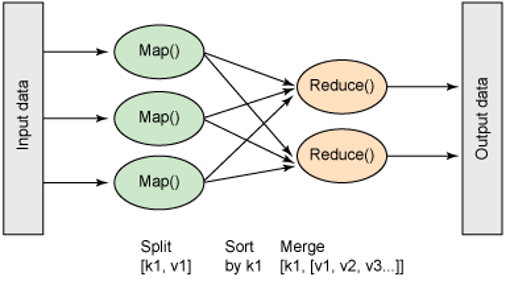
\includegraphics[width=0.55\linewidth]{mapreduce-diagram-by-ibm.png} \hfill \mbox{ }
\end{frame}

\begin{frame}{}
\LARGE
\vspace{1.25 cm}
\begin{center}
Physics and computing crossed paths in a different way.
\end{center}
\end{frame}

\begin{frame}{Physicists got into computers when they became general-purpose}
\vspace{0.5 cm}

\begin{columns}
\column{0.3\linewidth}
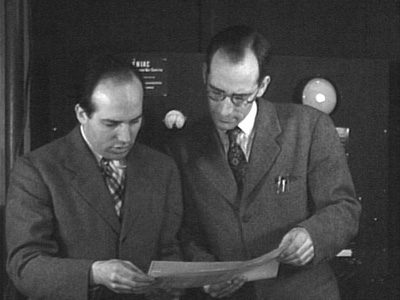
\includegraphics[width=\linewidth]{presper-and-mauchly.jpg}

\column{0.7\linewidth}
1944: John Mauchly (physicist) and J.\ Presper Eckert (electrical engineer) design ENIAC to replace mechanical computers.

\vspace{0.25 cm}
\uncover<2->{ENIAC was one of the first computers driven by machine code instructions, stored as a program in memory.}
\end{columns}

\vspace{0.25 cm}
\begin{uncoverenv}<3->
\begin{columns}
\column{0.65\linewidth}
1945: John von Neumann learned of their work and suggested using it for nuclear simulations (H-bomb).

\vspace{0.25 cm}
\uncover<4->{His internal memo describing ENIAC's stored programs was leaked; now known as ``Von Neumann architecture.''}

\vspace{0.25 cm}
\uncover<5->{Los Alamos group led by Nicholas Metropolis, developed Monte Carlo techniques for physics problems.}
\column{0.35\linewidth}
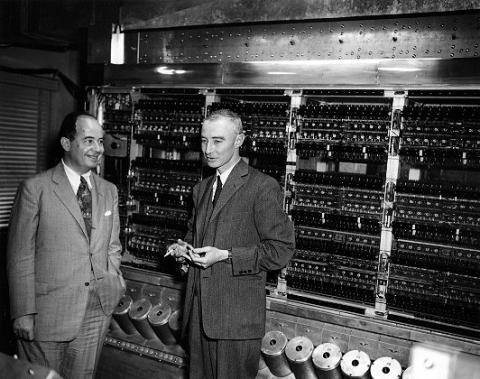
\includegraphics[width=\linewidth]{neumann_oppie.jpg}
\end{columns}
\end{uncoverenv}
\end{frame}

\begin{frame}{The actual programming was performed by six women}
\begin{columns}[t]
\column{0.15\linewidth}
\begin{center}
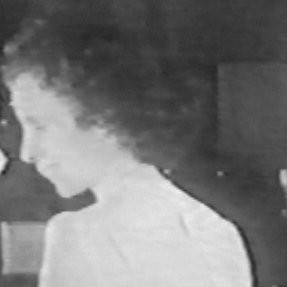
\includegraphics[width=\linewidth]{Kay-McNulty.jpg}

Kathleen McNulty
\end{center}

\column{0.15\linewidth}
\begin{center}
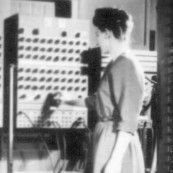
\includegraphics[width=\linewidth]{Fran-Bilas.jpg}

Frances Bilas
\end{center}

\column{0.15\linewidth}
\begin{center}
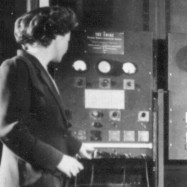
\includegraphics[width=\linewidth]{Betty-Jennings.jpg}

Betty Jean Jennings
\end{center}

\column{0.15\linewidth}
\begin{center}
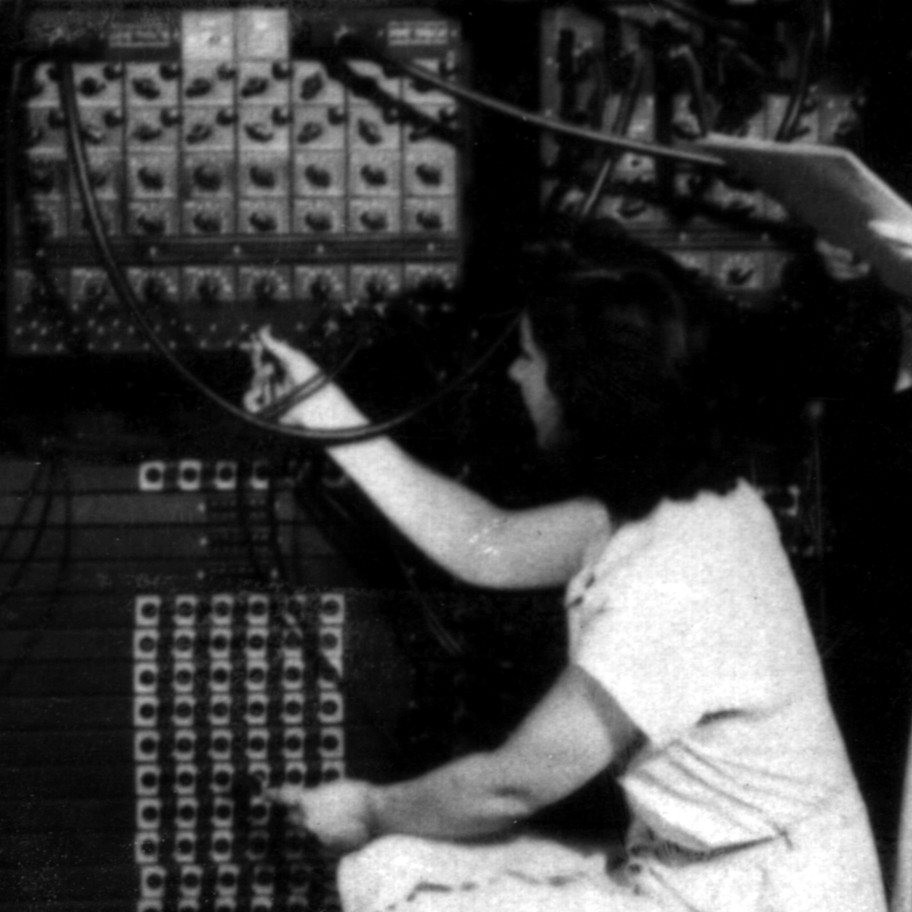
\includegraphics[width=\linewidth]{Ruth-Lichterman.jpg}

Ruth Lichterman
\end{center}

\column{0.15\linewidth}
\begin{center}
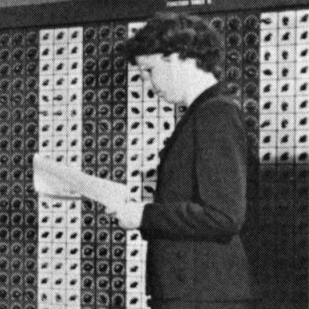
\includegraphics[width=\linewidth]{Betty-Snyder.jpg}

Elizabeth Snyder
\end{center}

\column{0.15\linewidth}
\begin{center}
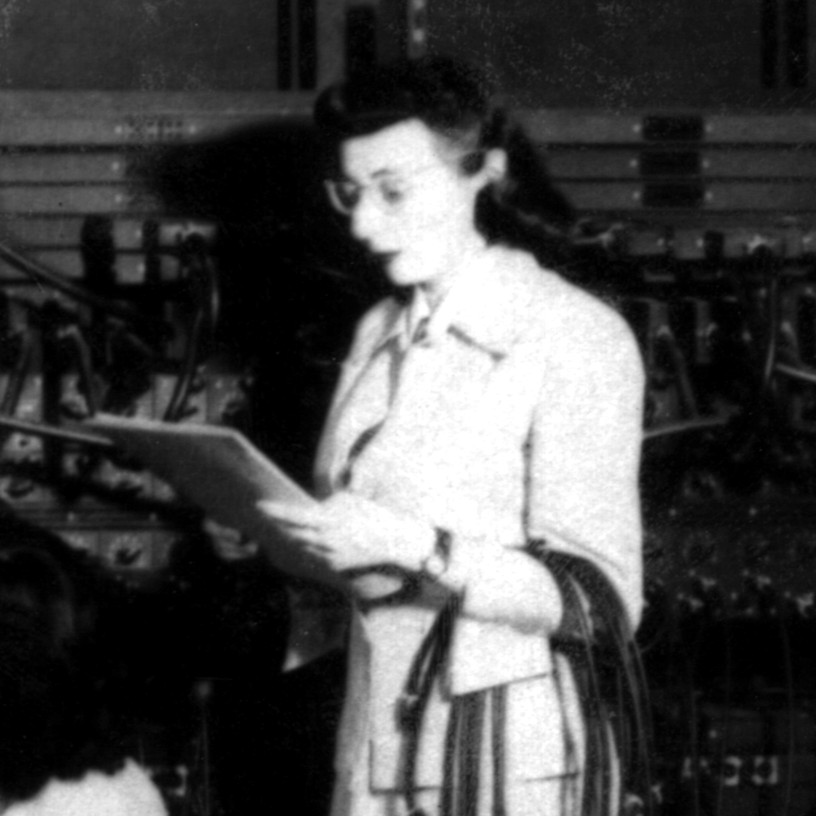
\includegraphics[width=\linewidth]{Marlyn-Meltzer.jpg}

Marlyn Wescoff
\end{center}
\end{columns}
\end{frame}

\begin{frame}[fragile]{Eckert-Mauchly Computer Corporation $\to$ Remington Rand}
\vspace{0.5 cm}

\begin{columns}
\column{0.7\linewidth}
Mauchly and Eckert ``went into industry'' selling computers; the first one (UNIVAC) to the U.S.\ Census.

\vspace{0.5 cm}
\begin{uncoverenv}<2->
1950: First executable high-level language, Short Code was a transliterated interpreter of mathematical formulas.
\begin{center}
\small
\vspace{-0.1 cm}
\begin{minipage}{0.8\linewidth}
\begin{verbatim}
math: X3 =  (  X1 +  Y1 )  /  X1 * Y1
code: X3 03 09 X1 07 Y1 02 04 X1   Y1
\end{verbatim}
\end{minipage}

\vspace{0.2 cm}
\normalsize
50$\times$ slower than machine code because it was interpreted.
\end{center}
\end{uncoverenv}

\vspace{0.5 cm}
\uncover<3->{1952--1959: Employee Grace Hopper develops a series of {\it compiled} languages, ultimately COBOL.}

\vspace{0.5 cm}
\uncover<4->{Meanwhile, IBM develops FORTRAN: 1954--1957.}

\column{0.3\linewidth}
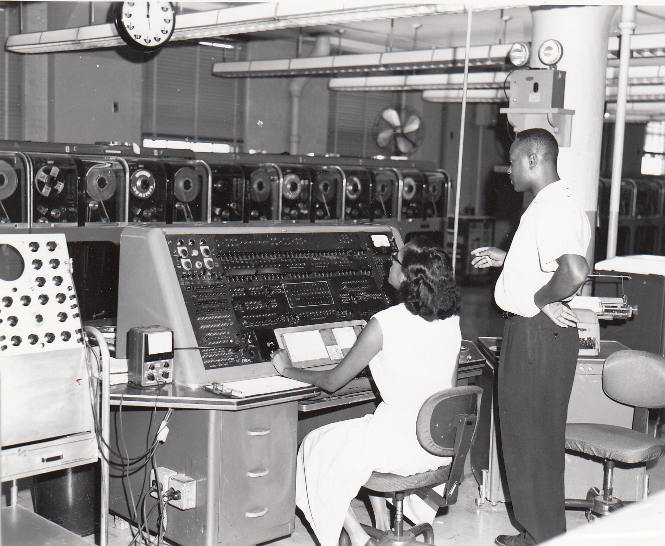
\includegraphics[width=\linewidth]{Univac_I_at_Census_Bureau_with_two_operators.jpg}

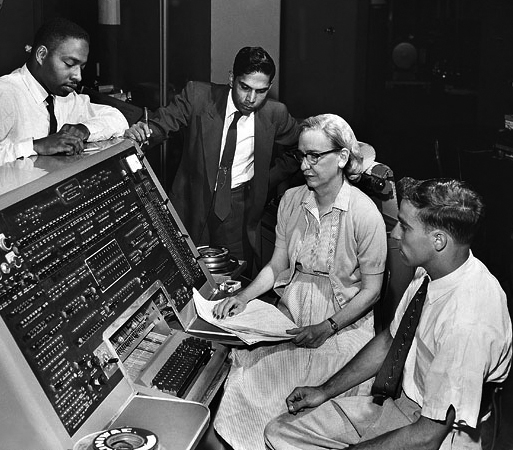
\includegraphics[width=\linewidth]{Grace_Hopper_and_UNIVAC.jpg}
\end{columns}
\end{frame}




\begin{frame}{}
\end{frame}





\end{document}
